



\chapter{Grundlagen der Bildverarbeitung und der Skalierung von Bildern}

\section{Einblick in die Bildverarbeitung}

Die Bildverarbeitung hat eine faszinierende Geschichte der Entwicklung und Innovation durchlaufen.
In den letzten Jahrzehnten hat sie sich zu einem zentralen Bereich der Künstlichen Intelligenz entwickelt.
In diesem Abschnitt werfen wir einen Blick auf die historische Entwicklung und den aktuellen Stand der Bildverarbeitung sowie mögliche zukünftige Entwicklungen.

Die Anfänge der Bildverarbeitung reichen zurück bis in die 1960er Jahre, als die theoretischen Grundlagen gelegt wurden\footfullcite{newell1963learning}.
In den 1980er Jahren erfolgte ein weiterer Boom mit dem Aufkommen von Expertensystemen\footfullcite{barr1981handbook}.
Doch erst in den letzten Jahren, insbesondere seit 2010, hat die Bildverarbeitung einen revolutionären Fortschritt erlebt, der auf den Durchbrüchen im Bereich des maschinellen Lernens beruht\footfullcite{ramachandram2017deep}.

\begin{figure}[h]
    \centering
    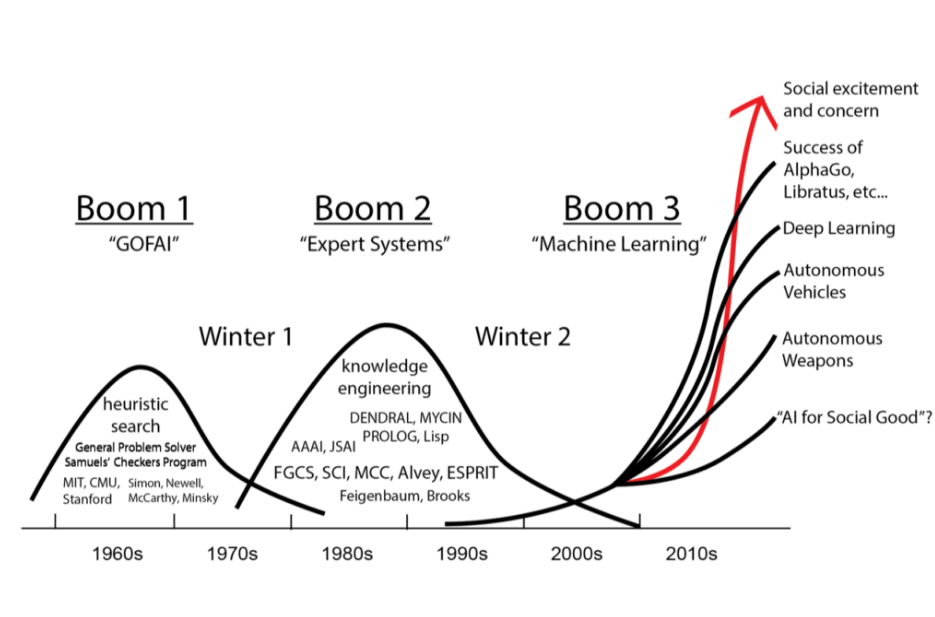
\includegraphics[width=0.8\textwidth]{img/history_bildverarbeitung.png}
    \caption{Die 3 Booms in der Geschichte von KI. Vorlesung DHBW Karlsruhe, TINF20, 2023 – D. Münch}
    \label{fig:history_bildverarbeitung}
\end{figure}

Die Geschichte der Künstlichen Intelligenz und der Bildverarbeitung ist eng miteinander verknüpft.
Bereits in den 1940er und 1950er Jahren wurden erste Modelle menschlicher Neuronen entwickelt, um die Funktionsweise des Gehirns besser zu verstehen\footfullcite{mcculloch1943logical}.
In den 1950er Jahren wurde die Künstliche Intelligenz als akademisches Fachgebiet etabliert, und es wurden erste Programme wie der "General Problem Solver" entwickelt.

In den 1960er Jahren wurde mit dem ADAptive LInear NEuron\footfullcite{specht1990probabilistic} (ADALINE) ein adaptives Mustererkennungssystem entwickelt, das als Meilenstein in der Bildverarbeitung gilt.
In den folgenden Jahrzehnten wurden zahlreiche mathematische Theorien und Methoden wie Hidden-Markov-Modelle\footfullcite{eddy2004hidden} (HMMs) und Data-Mining entwickelt, um die Bildverarbeitung weiter voranzutreiben.

Allerdings gab es auch Herausforderungen zu bewältigen. In der Vergangenheit waren die Trainingsdaten begrenzt und die Sensorik nicht ausgereift genug\footfullcite{kurzweil1990age}. Zudem waren die Rechenleistungen der Computer nicht ausreichend, um komplexe Aufgaben in Echtzeit zu bewältigen. Die Kombinatorik und Komplexität der Problemstellungen, wie beispielsweise die Gesichtserkennung, stellten weitere Schwierigkeiten dar.

In den letzten Jahren kam es zu einem regelrechten Revival der Künstlichen Intelligenz und der Bildverarbeitung\footfullcite{alom2018history}. Durch den Einsatz von Deep Learning und insbesondere von Deep Convolutional Neural Networks wie dem bahnbrechenden AlexNet im Jahr 2012 wurden große Fortschritte erzielt. So konnte beispielsweise im Jahr 2016 AlphaGo den Weltmeister im Spiel Go besiegen\footfullcite{hassabis2017artificial}. Allerdings brachten diese Entwicklungen auch neue Herausforderungen mit sich, wie beispielsweise die Entstehung von DeepFakes im Jahr 2017\footfullcite{kietzmann2020deepfakes}.

Der aktuelle Stand der Bildverarbeitung ist geprägt von einer beeindruckenden Leistungsfähigkeit und einer breiten Anwendungspalette. Doch die Möglichkeiten sind noch lange nicht ausgeschöpft. Zukünftige Entwicklungen könnten die Bildverarbeitung in Bereichen wie der Medizin, der Sicherheitstechnik und der Automatisierung weiter vorantreiben und neue Perspektiven eröffnen.

In diesem Kapitel werden wir uns mit den Grundlagen der Bildverarbeitung und der Skalierung von Bildern befassen, um ein solides Fundament für das weitere Verständnis dieses faszinierenden Bereichs zu schaffen.

\section{Skalierung von Bildern}

\subsection{Arten der Skalierungen: Interpolation und Skalierung}
    Die Interpolation und die Skalierung von Bildern oder Bildbereichen sind wichtige Konzepte der Bildverarbeitung. 
    Das Verfahren der Interpolation ermöglicht es neue Pixelwerte auf Basis vorgegebener Werte zu berechnen.
    Die Skalierung ist eine Anpassung der Bildgröße durch das Ändern der Anzahl von Pixeln oder der Auflösung. 
    
    Im Kontext der Bildverarbeitung wird Interpolation häufig verwendet, um die Größe von Bildern zu ändern, ohne dass dabei die Anzahl der Pixel verändert wird. Dazu werden neue Pixelwerte berechnet, indem vorhandene Pixelwerte interpoliert werden. 
    
    Die Wahl der Interpolationsmethode hat einen großen Einfluss auf die Qualität des interpolierten Bildes. 
    In der Bildverarbeitung gibt es verschiedene Interpolationsmethoden, wie z.B. Nearest-Neighbor-Interpolation, Bilineare Interpolation oder Bikubische Interpolation.
    Skalierung hingegen verändert die Größe eines Bildes, indem die Anzahl der Pixel oder die Auflösung verändert wird. 
    Im Gegensatz zur Interpolation wird die Anzahl der Pixel bei der Skalierung verändert, um das Bild kleiner oder größer zu machen. 
    Auch hier hat die Wahl der Skalierungsmethode einen großen Einfluss auf die Qualität des resultierenden Bildes.

\subsection{Bildformate}
    Einige Bildformate sind rasterbasiert und repräsentieren Bilder als Raster von einzelnen Punkten oder Pixeln. Sie ermöglichen eine detaillierte Darstellung, sind jedoch möglicherweise anfällig für Qualitätsverluste bei der Skalierung. Auf der anderen Seite verwenden andere Formate, wie Vektorgrafiken, mathematische Beschreibungen von Linien und Formen, was zu einer verlustfreien Skalierung führen kann und eine hohe Flexibilität bei der Bearbeitung bietet.
    In unsere Arbeit werden wir uns hauptsächlich auf die Verarbeitung von Raster-basierten Bildern umfassen.
    
    Historisch gesehen gab es jedoch viele unterschiedliche Formate für Bilder. 
    Zunächst erschufen unterschiedliche Softwareentwickler im Bereich der Bildverarbeitung häufig ihre eigenen Formate.\footfullcite{burger2009digitale}
    Einheitliche Standards, wie sie heute im Einsatz sind, etablierten sich erst später.
    Ein Vorreiter der modernen Bildformate ist das "Portable Network Graphics Format"\footfullcite{boutellpng}, das 1985 in den USA vorgestellt wurde. 
    Moderne Dateiformate zur Speicherung von Bildern werden anhand der Art des Bildes sowie der Kriterien Speicherbedarf und Kompression, Kompatibilität und ihrem Anwendungsbereich bewertet. 
    \footfullcite{burger2009digitale}
    
    \subsubsection{Portable Network Graphics Format}
        \acf{PNG} Format setzt einen besonderen Fokus auf eine geringe Komplexität und eine einfache Implementierung des Standards. 
        Der Standard kann frei von jedem genutzt werden.
        Des weiteren profitiert das Format von verlustfreier Kompression. \footfullcite{boutell1997png}
        \ac{PNG} unterstützt Vollfarbbilder, Grauwertbilder, Transparentz sowie Indexbilder. \footfullcite{burger2015digitale}
        Der \ac{PNG}-Algorithmus komprimiert Bilder, indem er mehrere Techniken, einschließlich Filterung und Huffman-Codierung anwendet. 
        Zunächst wird das Bild in Blöcke von 16 x 16 Pixeln aufgeteilt und dann wird auf jedem Block ein Filter angewendet, um Redundanzen zu entfernen. 
        Anschließend wird das Ergebnis der Filterung Huffman-codiert, um eine effiziente Darstellung der Daten zu erreichen.
        Characteristisch für PNG-Dateien ist auch die Möglichkeit, transparente Flächen einzubauen. 
        Der Standard verwendet eine spezielle Methode, um Transparenz darzustellen. 
        Diese wird als Alpha-Kanal bezeichnet und ermöglicht es, transparente sowie halbtransparente Bilder zu erstellen.
        Die kompekte Komprimmierung des PNG-Formats hat dafür gesorgt, dass der Standard im Internet eine hohe Beliebtheit genießt. 
        \footfullcite{w3c_png}
    
    \subsubsection{JPG-Format}

    Das \ac{JPG}-Format, auch bekannt als \ac{JPEG}, ist eines der am weitesten verbreiteten und bekanntesten Bildformate. Es wurde von der gleichnamigen Expertengruppe entwickelt und 1992 veröffentlicht.
    
    \ac{JPEG} basiert auf einer verlustbehafteten Kompressionsmethode, bei der Bildinformationen reduziert werden, um die Dateigröße zu verringern. Dies ermöglicht eine effiziente Speicherung und Übertragung von Bildern. Die Kompressionsrate kann je nach gewünschter Qualität und Dateigröße angepasst werden.
    
    Das \ac{JPEG}-Format eignet sich besonders gut für fotografische Bilder und komplexe Szenen mit vielen Farbverläufen und Details. Es unterstützt eine hohe Farbtiefe und kann Millionen von Farben darstellen. Aufgrund der verlustbehafteten Kompression können jedoch bei hohen Kompressionsraten Artefakte und Qualitätsverluste sichtbar werden.
    
    Das \ac{JPG}-Format ist weit verbreitet und wird von den meisten Bildbetrachtungs- und Bildbearbeitungsprogrammen unterstützt. Es ist auch das bevorzugte Format für Bilder im Internet, da es eine gute Balance zwischen Qualität und Dateigröße bietet. Es ist jedoch wichtig, die Kompressionsrate sorgfältig zu wählen, um ein optimales Ergebnis zu erzielen und Qualitätsverluste zu minimieren.
    
    Insgesamt ist das \ac{JPG}-Format eine beliebte Wahl für die Speicherung und Weitergabe von fotografischen Bildern, insbesondere wenn es auf eine effiziente Dateigröße und eine breite Kompatibilität ankommt.
            
    
    \subsubsection{Scalable Vector Graphics}
    \begin{quote}
        The main idea motivating \ac{SVG} was simple: to create a generic document-oriented solution  for graphics that can be adapted to modern media
        \grqq{}~\footfullcite{book:729077}
    \end{quote}
    %Evaluation und Implementierung eines Bildverarbeitungsverfahrens zur Füllstandsmessung
    Scalable Vector Graphics (SVG) steht für ein Format, das Vektorgrafiken basierend auf \ac{XML} darstellt.
    Im Gegensatz zu Rastergrafiken, wie z.B. PNG, die aus Pixeln bestehen und bei Vergrößerung an Schärfe verlieren, sind Vektorgrafiken vektorbasiert und behalten ihre Qualität bei beliebiger Skalierung. 
    Der Standard ermöglicht eine besonders effiziente Speicherung von Bildern.
    SVG ist außerdem ein offenes Format und unterstützt Interaktivität, Animation und Skripting.\footfullcite{quint2003scalable} 
    Da SVG auf XML basiert, kann es auch mit anderen Webtechnologien wie HTML, \ac{CSS} und JavaScript integriert werden.\footfullcite{mdn_svg} 
        
    \subsubsection{Weitere Standards}
        %TODO MEHR TEXT!!!! 
        \begin{description}
            \item[\ac{GIF}]~\\
                Ein Format für animierte Rastergrafiken mit einer begrenzten Farbpalette von 256 Farben. 
                Es verwendet eine verlustfreie Kompression, die aber nicht sehr effizient ist. 
                Es ist geeignet für einfache Animationen und Grafiken mit wenigen Farben.
            \item[\ac{TIFF}]~\\
                Ein Format für hochauflösende Rastergrafiken ohne Kompression oder mit verlustfreier Kompression.
                Es wird oft im Druckbereich verwendet, da es viele Optionen für Farbmanagement und Metadaten bietet.
                Es ist aber nicht sehr kompatibel mit Webbrowsern \\
            \item[\ac{PSD}]~\\
                Ein Format für Photoshop-Dokumente, das alle Ebenen, Masken, Effekte und andere Informationen speichert.
                Es ermöglicht eine umfangreiche Bearbeitung von Rastergrafiken, ist aber nur mit Photoshop kompatibel.\\
            \item[\ac{BMP}]~\\
                Ein Format für unkomprimierte Rastergrafiken mit hoher Qualität.
                Es wird selten verwendet, da es sehr große Dateien erzeugt und keine Transparenz oder andere Funktionen unterstützt. \\
            \item[\ac{EPS}]~\\
                Ein Format für vektorbasierte Grafiken, das Kurven, Texte und andere Elemente speichert.
                Es kann skaliert werden ohne Qualitätsverlust und wird oft im Druckbereich verwendet.
                Es ist aber nicht sehr kompatibel mit Webbrowsern oder anderen Programmen. \\
        \end{description}
        Weiterhin gibt es unzählige Standards um Grafiken darzustellen. Diese übersteigen jedoch den Umfang dieser Arbeit.
        \footfullcite{prepressure_file_formats}\footfullcite{ionos_file_formats}\footfullcite{rabbani2002overview}\footfullcite{marcellin2000overview}\footfullcite{britannica_jpeg}\footfullcite{elsevier_artwork}
\subsection{Wichtige Aspekte der Skalierung}
    \subsubsection{Segmentierung}
    
        Die Segmentierung von Bildern ist ein wichtiges Verfahren der Bildverarbeitung, da es ermöglicht, ein Bild in sinnvolle Regionen zu unterteilen. 
        Hierbei können verschiedene Verfahren, wie Schwellenwert- oder Clustering-Methoden eingesetzt werden. 
        Die Genauigkeit der Segmentierung hängt dabei maßgeblich von der Komplexität des Bildes und der gewählten Methode ab.
        Eine erfolgreiche Segmentierung kann für viele Anwendungen von Nutzen sein.
        Die automatischen Erkennung von Gesichtern oder die Identifizierung von Verkehrszeichen auf Straßenbildern sind die populärsten Beispiele.
        Jedoch ist es oft schwer genaue Grenzen zwischen Objekten in Bildern mit komplexen Strukturen zu erkennen.
    
    \subsubsection{Klassifizierung}
    
        Die Klassifizierung von Bildinhalten ist ein weiterer wichtiger Aspekt der Bildverarbeitung.
        Hierbei werden Bilder in automatisch bestimmte Kategorien eingeteilt. 
        Beispielanwendungen inkludieren das Erkennen von Tierarten auf Naturfotos oder das Identifizieren von Gesichtern auf Fotos. 
        Hierfür können verschiedene Techniken verwendet werden. Beispiele sind Deep Learning oder Entscheidungsbaum-Algorithmen.
        Eine erfolgreiche Klassifizierung kann für viele Anwendungen genutzt werden, wie zum Beispiel zur Automatisierung von Aufgaben oder im maschinellen Lernen. 
        Die Geneauigkeit einer Klassifizierung wird von Faktoren, wie zum Beispiel von der Qualität der Trainingsdaten oder der Komplexität der verwendeten Klassifikationsmethode beeinflusst.
    
    \subsubsection{Objekterkennung und -verfolgung}
    
        Die Objekterkennung und -verfolgung ist ein wichtiger Aspekt der Bildverarbeitung, der oft in Anwendungen wie der Überwachung und Robotik genutzt wird. 
        Hier geht es darum, Objekte in Bildern oder Videos zu erkennen und ihre Bewegungen zu verfolgen. 
        Es können verschiedene Techniken eingesetzt werden, wie zum Beispiel Hintergrundsubtraktion oder optische Flussberechnung.
        Eine erfolgreiche Objekterkennung und -verfolgung kann für viele Anwendungen genutzt werden, wie zum Beispiel in der Videoüberwachung oder bei der Steuerung von autonomen Fahrzeugen. 
        Allerdings gibt es auch Herausforderungen bei der Objekterkennung und -verfolgung, wie zum Beispiel die Bewältigung von Hintergrundrauschen oder die Verfolgung von Objekten bei hoher Geschwindigkeit.
    
    \subsubsection{3D-Bildverarbeitung}
        In der 3D-Bildverarbeitung werden dreidimensionale Bilder und Modelle analysiert und verarbeitet.
        Die Anwendungsfelder dieser Technologien reichen von medizinischen Umgebungen bis hin zur industriellen Fertigung.
        In bildgebenden medizinischen verfahren werden 3D-Bilder für die Diagnose von Krankheiten und Verletzungen verwendet. 
        In der industriellen Fertigung werden 3D-Modelle für die Qualitätssicherung und die Fehlererkennung verwendet.
    
    \subsubsection{Bildkompression}
        Da Bilder in der Regel große Datenmengen erzeugen, die für die Übertragung und Speicherung unpraktisch sind, benötigt es oft eine Bildkompression. 
        Durch Kompressionstechniken wie z.B. die JPEG-Kompression kann die Größe von Bildern erheblich reduziert werden ohne dabei große QUalitätsverluste zu erleiden.
    
\section{Echtzeitverarbeitung von Bildern}

    Die Echtzeitverarbeitung von Bildern stellt eine Herausforderung in der Bildverarbeitung dar, da sie eine sehr schnelle Verarbeitung erfordert, um zeitkritische Anwendungen wie autonomes Fahren oder Augmented Reality in Echtzeit zu realisieren.\footfullcite{zhang2018scalable}$^{,}$\footfullcite{li2020convolutional}
    Bei diesen Aufgaben müssen Bilder in Echtzeit erfasst, verarbeitet und angezeigt werden, um eine reibungslose Funktionalität zu gewährleisten.
    
    Unter Echtzeitverarbeitung versteht man die Fähigkeit, Daten sofort und unmittelbar zu verarbeiten, ohne wahrnehmbare Verzögerungen.
    In Bezug auf die Bildverarbeitung bedeutet dies, dass die Verarbeitung innerhalb eines bestimmten Zeitrahmens erfolgen muss, um den Anforderungen der Anwendung gerecht zu werden.
    In der Regel ist dies eine Echtzeitverarbeitung in Echtzeit oder nahezu Echtzeit.
    
    Die Echtzeitverarbeitung von Bildern erfordert in der Regel eine hohe Rechenleistung, um die Daten schnell genug zu verarbeiten.
    Hierbei kommen spezielle Algorithmen und Techniken zum Einsatz, die für eine effiziente Verarbeitung sorgen.
    Beispielsweise werden häufig spezialisierte Hardware wie Grafikprozessoren (GPUs) oder FPGA (Field Programmable Gate Array)-basierte Systeme verwendet, um die Verarbeitungsgeschwindigkeit zu erhöhen.
    
    Eine weitere Herausforderung bei der Echtzeitverarbeitung von Bildern ist die Echtzeit-Kommunikation zwischen den verschiedenen Komponenten des Systems.
    Hierbei müssen Daten schnell und zuverlässig ausgetauscht werden, um Verzögerungen zu vermeiden. Hierfür kommen häufig spezielle Systeme zum Einsatz, die für eine schnelle Übertragung und parallele Verarbeitung von Daten optimiert sind.
    Eine effiziente Datenübertragung und Kommunikation zwischen den einzelnen Komponenten des Systems ist entscheidend, um eine Echtzeitverarbeitung zu ermöglichen.\footfullcite{oehlrich1992transputersystem}
    
    Insgesamt erfordert die Echtzeitverarbeitung von Bildern eine Kombination aus leistungsstarker Hardware, effizienten Algorithmen und einer effektiven Datenkommunikation, um die Anforderungen zeitkritischer Anwendungen zu erfüllen.
    Durch den Fortschritt in der Hardware- und Softwaretechnologie wird die Echtzeitverarbeitung von Bildern immer besser und ermöglicht somit eine Vielzahl von spannenden Anwendungen.
    
\section{Anwendungen von Skalierungsmethoden}
    % help
    Die Anwendung von Skalierungsmethoden bietet eine Vielzahl ungewöhnlicher, aber äußerst nützlicher Anwendungen in verschiedenen Sektoren.
    In der Landwirtschaft können diese Methoden dazu beitragen, die Gesundheit von Pflanzen zu überwachen und den Einsatz von Pestiziden zu optimieren.
    Durch die Analyse von Pflanzenbildern können frühzeitig Krankheiten erkannt und gezielte Maßnahmen ergriffen werden, um Ernteausfälle zu minimieren.
    In der Archäologie ermöglichen Skalierungsmethoden die digitale Rekonstruktion verwitterter oder beschädigter Artefakte.
    Dies eröffnet Forschern neue Einblicke in die Geschichte vergangener Zivilisationen und ermöglicht die Erstellung interaktiver virtueller Museen.
    In der Modeindustrie ermöglichen Skalierungsmethoden das virtuelle Anprobieren von Kleidung, was den Kunden die Möglichkeit gibt, Passform und Aussehen der Kleidungsstücke im Voraus zu überprüfen und das Online-Shopping-Erlebnis zu verbessern.
    Durch die Integration von Bildverarbeitung und Augmented Reality entsteht eine innovative und interaktive Shopping-Erfahrung.
    Insgesamt bieten Skalierungsmethoden in diesen verschiedenen Sektoren ungewöhnliche Anwendungen, die zu Effizienzsteigerungen, Erkenntnisgewinnen und verbesserten Kundenerfahrungen führen.
